% !TEX root = ../main.tex
\subsubsection{Strong Coupling Constant $\alpha_s$}
\label{sssec::strong_coupling_constant}
    Measuring the experimental value of $\alpha_s$ is crucial for perturbative QCD calculations.
    To achieve this, the overall scale of renormalization needs to be determined.
    Typically, the mass of the neutral Bose particle $Z^0$, which is $91.19$ GeV, is chosen as the scale.
    Furthermore, the renormalization scheme should be fixed, which defines the coupling constant at a specific scale.
    The experimental results for $\alpha_s$ can be seen in Figure \ref{fig::alpha_q_dependence}.

    \begin{figure}[b!]
        \centering
        \frame{
        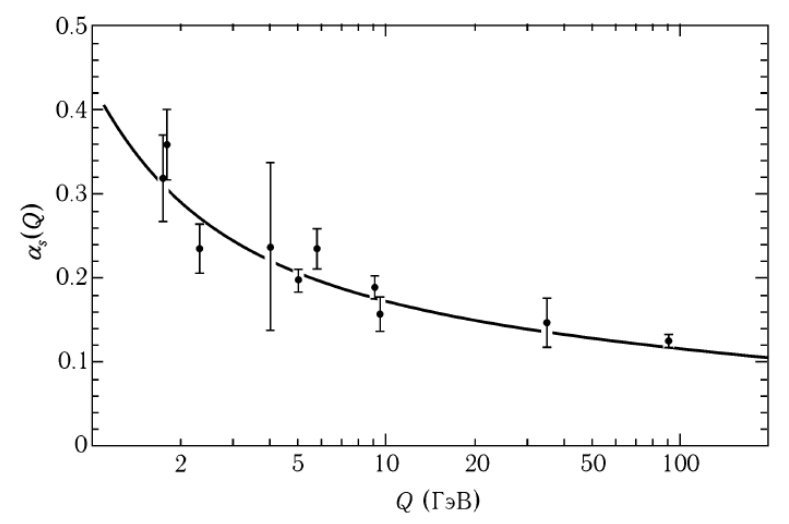
\includegraphics[width=0.8\textwidth]{13strong_coupling_constant_q.png}}
        \caption[$\alpha_s$ dependence on $Q^2$.]{Experimentally measured dependence of $\alpha_s$ on $Q$.
        The measured values are compared with the theoretical predictions of renormalized evolution with an initial value of $\alpha_s(m_z) = 0.117$ GeV.} % NOTE. Can't find a source :(.
        \label{fig::alpha_q_dependence}
    \end{figure}
